\section{Current Tumor Bed Localization Devices and Methods\label{sec:literatureReview:currentMethods}}

\hl{This could possibly go in background instead.\\}
Current devices and methods used for TB delineation include titanium, gold, or liquid fiducial markers/surgical clips, surgeon discretion, seroma formation, or implantable devices~\cite{RefWorks:RefID:25-acree2022review}.

\subsection{Fiducial Markers and Surgical Clips\label{sec:literatureReview:currentMethods:fiducialMarkers}}
Fiducial markers are solid metal clips inserted around the border of a tumor cavity immediately following the tumor removal~\cite{RefWorks:RefID:358-nihdefining}. These provide a 2D point mapping of the tumor space as shown below in Figure~\ref{fig:literatureReview:imaging_of_fiducal_clips_in_phantom_breast}.

Liquid fiducial markers were first used as spacers for prostate cancer treatment planning. They have since been repurposed to be used for TB delineation. These markers provide a clearer delineation than solid clips as they conform to the tumor cavity shape~\cite{RefWorks:RefID:25-acree2022review}.

\begin{figure}[H]
        \centering
        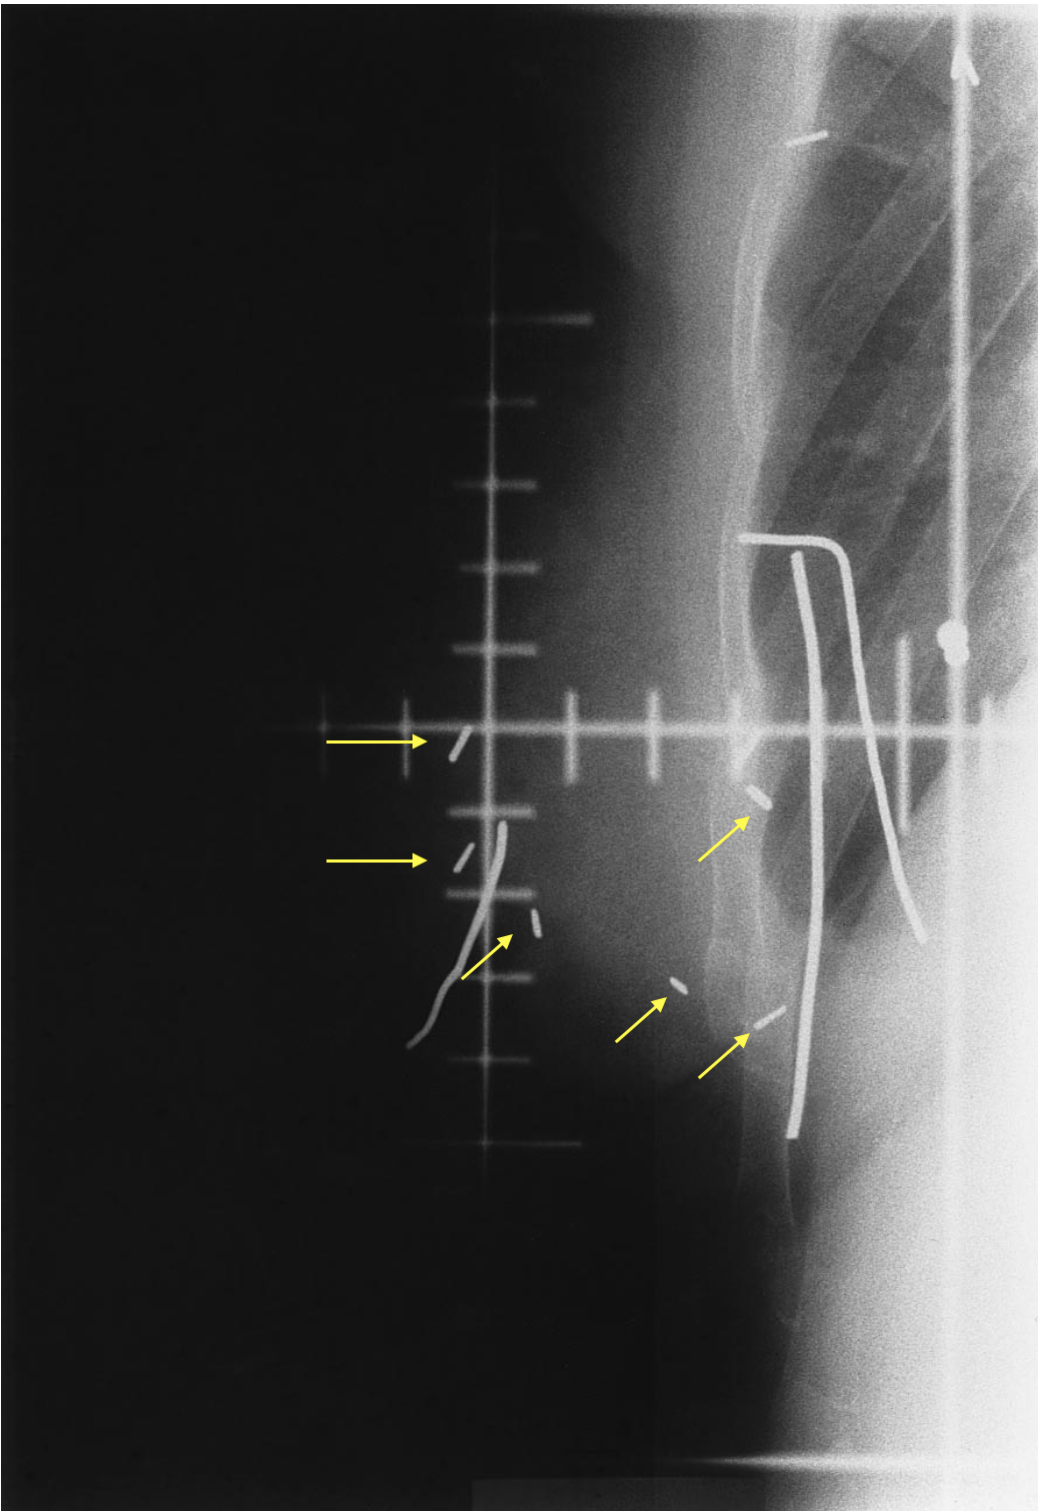
\includegraphics[height=0.3\textheight]{../figs/literature_review/imaging_of_fiducal_clips_in_phantom_breast.png}
        \caption{Imaging of Fiducial Clips in Phantom Breast. Yellow arrows indicate fiducial clips placed around tumor cavity. Adapted from \cite{RefWorks:RefID:178-krawczyk1994importance}.}
        \label{fig:literatureReview:imaging_of_fiducal_clips_in_phantom_breast}
\end{figure}

\subsection{Seroma Formation\label{sec:literatureReview:currentMethods:seromaFormation}}
\hl{Add more here about seromas}
Review of current accepted...\cite{RefWorks:RefID:25-acree2022review} has great stats on this (see Figure~\ref{fig:literatureReview:seromaFormationStats}).
\begin{figure}[h]
        \centering
        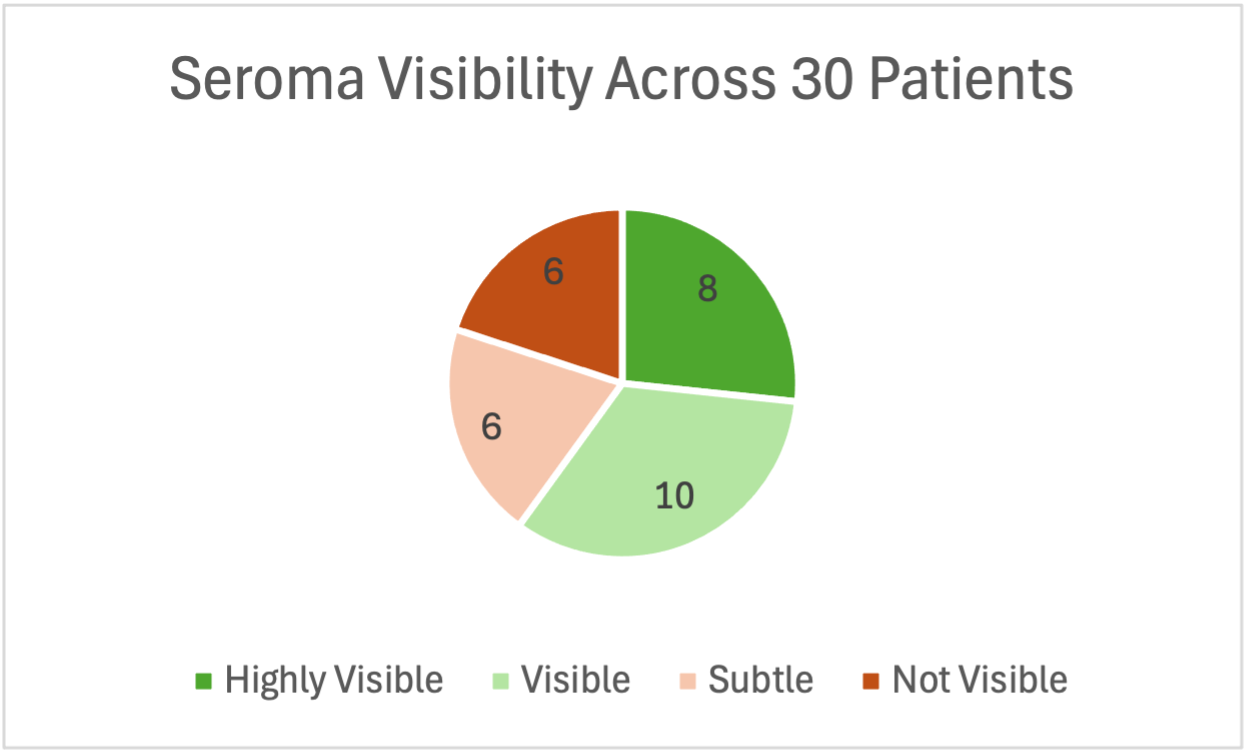
\includegraphics[width=0.7\textwidth]{../figs/literature_review/seroma_visibility_study_results.png}
        \caption{Statistics on Seroma Formation from \cite{RefWorks:RefID:25-acree2022review}.}
        \label{fig:literatureReview:seromaFormationStats}
\end{figure}

Using seroma formation to mark the tumor bed for radiation therapy involves outlining the seroma that forms following a lumpectomy procedure~\cite{RefWorks:RefID:25-acree2022review}.

\subsection{Implantable Devices\label{sec:literatureReview:currentMethods:implantableDevices}}
Lastly, implantable devices can be used to mark the tumor bed. One example is BioZorb (Hologic) which is a 3-dimensional coil-like structure with titanium clips embedded. This device is implanted into the tumor cavity following a lumpectomy procedure and improves on titanium clips alone by creating a 3D outline of the tumor bed. BioZorb was also designed to be reabsorbed into the body within a year~\cite{RefWorks:RefID:25-acree2022review}. BioZorb is shown below in Figure~\ref{fig:literatureReview:biozorb_implant}.
\begin{figure}[h!]
        \begin{minipage}{0.92\textwidth}
                \centering
                \begin{subfigure}[b]{0.9\textwidth}
                        \centering
                        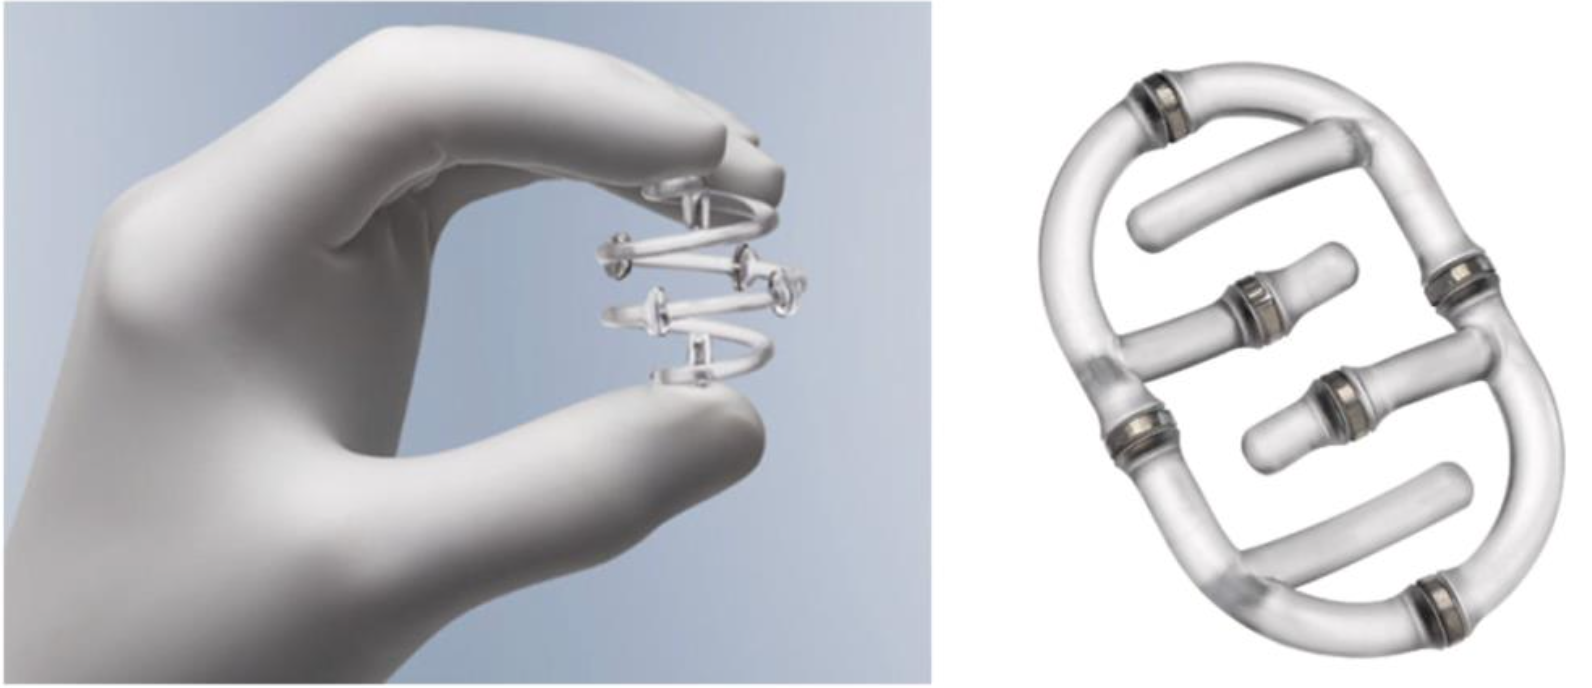
\includegraphics[width=\textwidth]{../figs/literature_review/BioZorb_physically.png}
                        \caption{BioZorb physically (top).}
                        \label{fig:literatureReview:biozorb_physically}
                \end{subfigure}

                \vspace{1em} % optional space between images

                \begin{subfigure}[b]{0.9\textwidth}
                        \centering
                        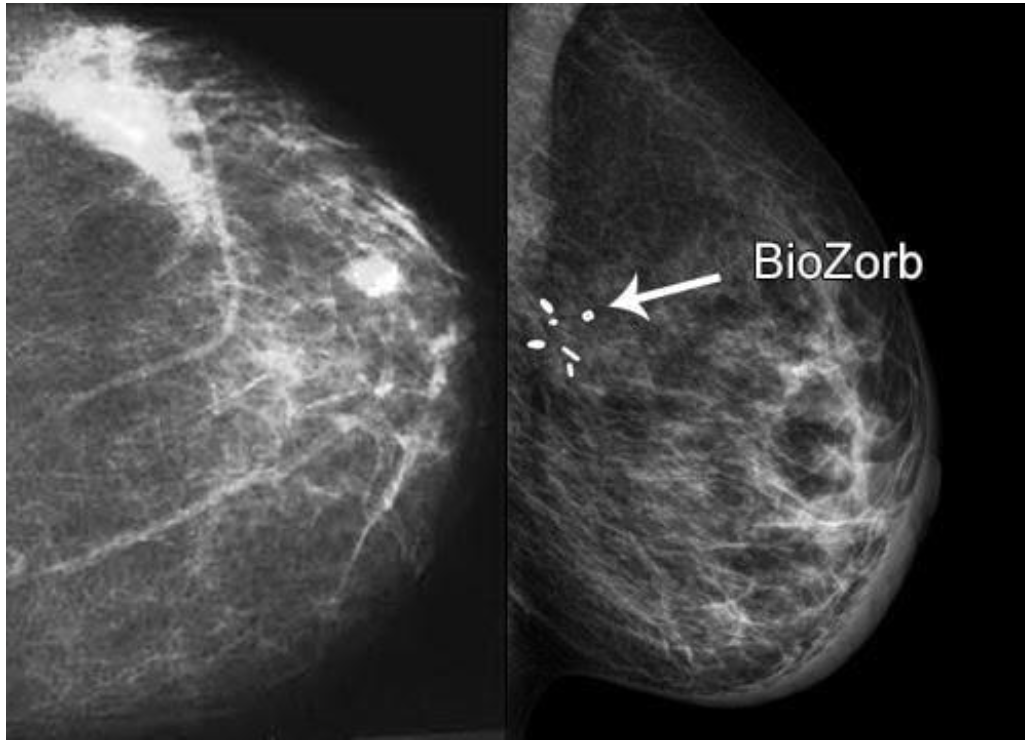
\includegraphics[width=\textwidth]{../figs/literature_review/BioZorb_in_imaging.png}
                        \caption{BioZorb in imaging.}
                        \label{fig:literatureReview:biozorb_in_imaging}
                \end{subfigure}
        \end{minipage}
        \caption{BioZorb, an implantable device to assist with TB delineation~\cite{RefWorks:RefID:370-einsteinisaac}.}
        \label{fig:literatureReview:biozorb_implant}
\end{figure}

\subsection{Veraform\label{sec:literatureReview:currentMethods:veraform}}
A newer implantable device is Veraform, a continuously radiographically opaque filament that is stitched around the tumor cavity. By being malleable and sewn in place, this device addresses space limitations and migration issues present in other devices~\cite{RefWorks:RefID:344-mitchell2019adaptable}. A simulation showing Veraform in use is shown below in Figure~\ref{fig:literatureReview:veraform_implant}.
\begin{figure}[h!]
        \centering
        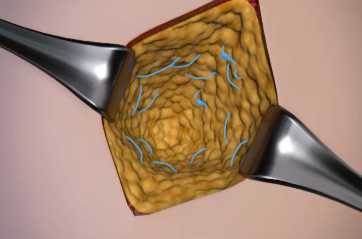
\includegraphics[width=0.6\textwidth]{../figs/literature_review/veraform_implant.png}
        \caption{Veraform, an implantable device to assist with TB delineation~\cite{RefWorks:RefID:344-mitchell2019adaptable}.}
        \label{fig:literatureReview:veraform_implant}
\end{figure}

\subsection{Challenges with Current Devices and Methods\label{sec:literatureReview:currentMethods:challengeswithcurrentdevicesandmethods}}

\hl{See if this could use more detail.}
\subsubsection{Challenges with Fiducial Markers\label{sec:literatureReview:currentMethods:challengeswithcurrentdevicesandmethods:fiducialMarkers}}
There are many challenges and inaccuracies that can result from using fiducial markers or surgical clips to create a TB volume. They provide single points of reference which can lead to inaccurate boundaries being drawn, there is no standardized recommendation of how many clips should be used, and clips can migrate over time leading to inaccurate TB localization~\cite{RefWorks:RefID:344-mitchell2019adaptable}. Migration is especially common when patients undergo oncoplastic reconstruction surgery following the lumpectomy procedure. In 2022, it was found the 30,000 breast-conserving therapy patients annually undergo oncoplastic reconstruction surgery~\cite{RefWorks:RefID:25-acree2022review}.

Another concern of surgical clips or fiducial markers is if a re-excision is required. This is when a margin of tissue removed during the lumpectomy is found to contain cancerous cells. When this is the case, a large enough margin surrounding the tumor was not removed, and a re-excision has to be made to remove additional margins. When markers are placed initially, these re-excisions can impact the accuracy of the initial marker placement. It was found that 10\% to 20\% of patients undergoing breast-conserving surgery require a re-excision~\cite{RefWorks:RefID:25-acree2022review}.

\subsubsection{Challenges with Seroma Formation\label{sec:literatureReview:currentMethods:challengeswithcurrentdevicesandmethods:seroma}}
\hl{Show change in seroma over time visual.\\}

Utilizing seroma formation can be unreliable, as the seroma may not always be localized to the tumor bed, relies on the excision closure method, and time elapsed after surgery\cite{RefWorks:RefID:25-acree2022review}. A seroma may represent the tumor bed, part of the tumor bed, or the entire area in which surgery was performed~\cite{RefWorks:RefID:344-mitchell2019adaptable}.

\subsubsection{Challenges with Biozorb\label{sec:literatureReview:currentMethods:challengeswithcurrentdevicesandmethods:biozorb}}
Biozorb was found to provide limited value to patients relative to its high cost~\cite{RefWorks:RefID:344-mitchell2019adaptable}. Additionally, Biozorb was also recalled due to patient discomfort, seroma formation, device migration, and failures to resorb into the body in the designated timeframe~\cite{RefWorks:RefID:296-2024hologic},~\cite{RefWorks:RefID:28-nudelunited}.
% \section{Current Tumor Bed Localization Devices and Methods\label{sec:literatureReview:currentMethods}}
% Summarize current clinical methods for localizing the tumor bed post-lumpectomy.
% Include fiducial markers, seroma tracking, and implantable devices (e.g., VeraForm).
% Discuss key limitations such as migration, resorption, visibility on imaging, and biocompatibility issues.

% \subsection{Challenges with Current Devices\label{sec:literatureReview:currentMethods:challenges}}
% Highlight why new localization methods are being explored.
% Cover limitations in accuracy, ease of placement, imaging visibility, and patient comfort.

\section{Extrusion Processes and Parameters\label{sec:literatureReview:extrusion}}
% Introduce extrusion in polymer processing and its relevance to filament production.

\subsection{Tabletop Extrusion Mechanics\label{sec:literatureReview:extrusion:mechanics}}
% Describe barrel, screw, hopper, nozzle, and drive systems.
% Discuss typical lab-scale extruders such as 3Devo or Filabot.

\subsubsection{Important Parameters\label{sec:literatureReview:extrusion:mechanics:parameters}}
% Detail process parameters:
% heat zones, material size/uniformity, screw RPM, cooling rate, pre-drying requirements, and melt flow index.

\subsection{Possible Issues with Extruding\label{sec:literatureReview:extrusion:issues}}
% Detail potential issues: clumping at hopper, clogging during extrusion, or inconsistent extrusion.

\subsection{Extruding Regrind\label{sec:literatureReview:extrusion:regrind}}
% Discuss reprocessing of polymer waste or failed prints.

\subsubsection{Machines for Creating Regrind\label{sec:literatureReview:extrusion:regrind:machines}}
% Mention industrial grinders, the Felfil Shredder, and similar tabletop systems.

\subsubsection{Challenges Extruding Regrind\label{sec:literatureReview:extrusion:regrind:challenges}}
% Problems include variable shape:
% 3Devo feeder or other vibration motors can help with these issues
% Felfil Shredder created a sieve to only use <=5x5mm pieces
% Find the one paper that analyzed different sizes to use

\subsubsection{Effects of Re-Extruding Materials\label{sec:literatureReview:extrusion:regrind:effects}}
% Discuss degradation, viscosity changes, and mechanical property shifts.

\subsection{Powder Extrusions\label{sec:literatureReview:extrusion:powder}}
% Discuss issues with powder extrusion: clumping, inconsistent back pressure, and variable flow rate.
% 3Devo feeder or other vibration motors can help with these issues

\subsection{Purging an Extruder\label{sec:literatureReview:extrusion:purging}}
% Explain the importance of regular purging to maintain extrusion quality and prevent contamination.

\subsubsection{Importance of Regular Purging\label{sec:literatureReview:extrusion:purging:importance}}
% Note 3Devo’s recommendation to purge monthly or whenever powder is used.
% Emphasize cleaning the barrel, removing contaminants, and ensuring uniform extrusion.

\subsubsection{Purging Procedures\label{sec:literatureReview:extrusion:purging:procedures}}
% Summarize cleaning methods:
% - Devoclean MT
% - Dyna-Purge series (L, K, D2)
% Include stepwise details from manufacturer documentation.

\subsubsection{Purging Compounds\label{sec:literatureReview:extrusion:purging:compounds}}
% Compare compound types, composition, and use cases.

\paragraph*{Vendors}
% Devoclean MT, Dyna-Purge L (soft), K (soft but abrasive), D2 (hard and abrasive).

\paragraph*{Material Compatibility}
% Discuss melt flow index and temperature matching to extruded materials.
% Note when harder materials (e.g., HDPE) are required to flush the purging compound.

\section{3D Printing Processes\label{sec:literatureReview:printing}}
% Introduce additive manufacturing context for polymer device fabrication.

\subsection{Fused Deposition Modeling (FDM)\label{sec:literatureReview:printing:FDM}}
% Describe the principle of FDM, typical materials, and its advantages over other AM methods.

\subsubsection{Important Parameters\label{sec:literatureReview:printing:FDM:parameters}}
% Discuss bed temperature, nozzle temperature, print speeds, and nozzle size/material.

\subsubsection{Optimal Printing Parameters\label{sec:literatureReview:printing:FDM:optimalParameters}}

\paragraph*{Calibrating Materials}
% Discuss calibration approaches such as for Prusa or Bambu to determine optimal print parameters
% Line test, calibration cube, temp tower, Bambu inherent calibrations

% Include recommended printing parameters for PLA, PCL, and PLCL.
\paragraph*{PLA Optimal Printing Parameters}

\paragraph*{PCL Optimal Printing Parameters}

\paragraph*{PLCL Optimal Printing Parameters}

\section{Creating PLCL Blends\label{sec:literatureReview:PLCL}}
% Introduce PLCL copolymer—its rationale, applications, and optimal ratio (70/30 PLA/PCL).

\subsection{Effects of Co-Polymer Composition\label{sec:literatureReview:PLCL:composition}}
% Detail the effects of different PLA/PCL compositions to help show why 70/30 is the best choice

\subsection{Synthesis Methods\label{sec:literatureReview:PLCL:synthesis}}
% Compare ring-opening polymerization (ROP) and block synthesis routes.

\subsection{Blending Techniques\label{sec:literatureReview:PLCL:blending}}
% Discuss melting methods (thermal) and solvent-based blending (chloroform or DCM).

\subsubsection{Injection Molding\label{sec:literatureReview:PLCL:blending:injectionMolding}}
% Explain how injection molding can melt the materials together but doesn't mix them well (maybe the lack of mixing will go in discussion if I can't find papers and am only basing that off of Rachmat's opinion).

\subsubsection{Extruding Raw Materials Together\label{sec:literatureReview:PLCL:blending:coextrusion}}
% Differentiate between single-screw and twin-screw extruders in blend formation.

\section{Alternative Device Fabrication Approaches\label{sec:literatureReview:alternativeDevices}}
% Review non-traditional or hybrid manufacturing strategies.
% Explored to see if there were better options than extruding a custom composite filament

\subsection{Composite Filaments\label{sec:literatureReview:alternativeDevices:compositeFilaments}}
% Summarize existing composite filaments, filler materials, and performance characteristics.

\subsection{Embedded Printing\label{sec:literatureReview:alternativeDevices:embeddedPrinting}}
% Discuss embedded printing (dropping clips inside print)

\subsection{Multi-Material Printing\label{sec:literaturereview:alternativeDevices:multiMaterialPrinting}}
% Discuss multi-material printing
% Show AMS (Bambu) and MMU (Prusa)
% Reference: \url{https://www.sciencedirect.com/science/article/pii/S1120179722020518}

\section{Radiopaque Agents\label{sec:literatureReview:radiopaque}}
% Discuss why radiopaque agents are used and their impact on imaging visibility.
% Radiopacity section in RefWorks

\subsection{Existing Radiopaque Filaments\label{sec:literatureReview:radiopaque:filaments}}
% Reference materials and data from Radiopaque Materials section in RefWorks.

\section{Imaging Studies\label{sec:literatureReview:imaging}}
% Summarize imaging studies assessing radiopacity and HU quantification.

\subsection{Interpreting Hounsfield Units\label{sec:literatureReview:imaging:HU}}
% Explain how HU correlates to material density and imaging contrast.

\subsection{Test Standards\label{sec:literatureReview:imaging:standards}}
% Mention ASTM F640-20 and similar standards for CT evaluation (Ref ID 342)

\subsection{Prior Studies\label{sec:literatureReview:imaging:priorStudies}}
% Include references such as Ref ID 77 for comparable imaging validation studies.

\section{Material Properties\label{sec:literatureReview:materials}}
% Review mechanical and physical properties of both biological and polymeric materials.

\subsection{Breast Tissue Properties\label{sec:literatureReview:materials:breast}}
% Summarize adipose and glandular tissue properties relevant to implant design.

\subsection{Polymer Properties\label{sec:literatureReview:materials:polymers}}
% Compare PLA, PCL, and PLCL mechanical and thermal characteristics.

\subsection{Effects of BaSO\textsubscript{4} Additives\label{sec:literatureReview:materials:BaSO4}}
% Discuss how radiopaque fillers influence modulus, brittleness, and imaging response.

\section{Mechanical Testing\label{sec:literatureReview:testing}}
% Explain standards, specimen design, and relevance to material characterization.

\subsection{Testing Standards\label{sec:literatureReview:testing:standards}}
% Include ASTM D638 (tensile) and D790 (flexural).

\subsection{Specimen Development\label{sec:literatureReview:testing:specimens}}
% Note using Type-V tensile bars (ASTM D638) due to limited material.
% Discuss 100\% infill rationale to eliminate void-based variability and effects of infill % on strength of material.

\subsection{Importance of Mechanical Testing\label{sec:literatureReview:testing:importance}}
% Explain what tensile strength, elastic modulus, and flexural modulus indicate about structure–property relationships.

\section{Characterizing Polymer Blends\label{sec:literatureReview:characterization}}
% Summarize analytical methods used to verify polymer composition and structure.

\subsection{NMR Testing\label{sec:literatureReview:characterization:NMR}}
% Discuss NMR for quantifying PLA/PCL ratio and copolymer composition.

\subsubsection{Powder Preparation\label{sec:literatureReview:characterization:NMR:powderPrep}}
% Compare mortar and pestle, ball milling, and 3D printed filament grinding.

\subsection{Microscopy\label{sec:literatureReview:characterization:microscopy}}
% Include optical and scanning electron microscopy for morphological analysis.

\subsection{Gel Permeation Chromatography (GPC)\label{sec:literatureReview:characterization:GPC}}
% Review methods for determining molecular weight distribution and polymer degradation.

\section{Project Road Mapping\label{sec:literatureReview:roadmap}}
% Explore literature on project visualization and management tools in research.

\subsection{Effects of Gantt Charts\label{sec:literatureReview:roadmap:gantt}}
% Discuss visualization, planning, and coordination benefits of Gantt charting.

\subsection{Other Visual Road Mapping Tools\label{sec:literatureReview:roadmap:otherTools}}
% Mention software and visual approaches beyond Gantt (Kanban, network maps, etc.).

\section{Belt Tensioning Systems\label{sec:literatureReview:beltTension}}
% Review mechanical belt tensioning designs in extrusion and motion systems.

\subsection{Inside vs Outside Idler Pulley\label{sec:literatureReview:beltTension:idler}}
% Compare idler pulley placements and performance implications.
% Reference: \url{https://www.barbieribelt.com/news/commonly-used-tensioning-methods-for-timing-belts}
